%
% File acl2021.tex
%
%% Based on the style files for EMNLP 2020, which were
%% Based on the style files for ACL 2020, which were
%% Based on the style files for ACL 2018, NAACL 2018/19, which were
%% Based on the style files for ACL-2015, with some improvements
%%  taken from the NAACL-2016 style
%% Based on the style files for ACL-2014, which were, in turn,
%% based on ACL-2013, ACL-2012, ACL-2011, ACL-2010, ACL-IJCNLP-2009,
%% EACL-2009, IJCNLP-2008...
%% Based on the style files for EACL 2006 by 
%%e.agirre@ehu.es or Sergi.Balari@uab.es
%% and that of ACL 08 by Joakim Nivre and Noah Smith

\documentclass[11pt,a4paper]{article}
\usepackage[hyperref]{acl2021}
\usepackage{times}
\usepackage{latexsym}
\renewcommand{\UrlFont}{\ttfamily\small}
\usepackage{graphicx}
% This is not strictly necessary, and may be commented out,
% but it will improve the layout of the manuscript,
% and will typically save some space.
\usepackage{microtype}

\aclfinalcopy % Uncomment this line for the final submission

%\setlength\titlebox{5cm}
% You can expand the titlebox if you need extra space
% to show all the authors. Please do not make the titlebox
% smaller than 5cm (the original size); we will check this
% in the camera-ready version and ask you to change it back.

\newcommand\BibTeX{B\textsc{ib}\TeX}

\title{Risks in using Intermediate Data for Domain Transfer Between Similar Domains}

\author{Nicolaj Valsted, Noah Syrkis, Tim Poulsen \\
  IT University of Copenhagen\\
  \eml{ \{nicv, nobr, timp\} @itu.dk}
}

\date{}
\begin{document}
\maketitle
\begin{abstract}

As unlabelled data sets become more common, the methods for learning from them become more relevant.
Semi-supervised learning, and more specifically self-training, is one such type of method applicable when labelled data from a similar domain is available.
If the domain differences are sufficiently large, intermediate data, similar to both source and target, might sustain the generalisation across the transfer, according to new research.
We explore whether there are risks to this approach, by using it on domains that have small differences and thus cannot be expected to benefit from the procedure.
We observe that under certain circumstances, our model is indeed negatively affected by the inclusion of intermediate data.
These findings are not particularly surprising, as introducing intermediate data between domains that already have considerable overlap, seems likely to only become a source of noise. Our project repository can be found at \url{https://github.com/syrkis/bridger}.

\end{abstract}

\section*{Introduction}
As natural language processing (NLP) becomes more broadly applied, the frequency with which raw, unlabelled training data is the best available, can be expected to increase.
Methods based on such data fall under the category of unsupervised or semi-supervised learning. 

In some instances, one has labelled data from a comparable domain to that of the unlabelled target domain. In such situations, it often makes sense to train on the labelled domain, and then transfer the generalised knowledge to the target, using methods such as self-training \cite{yarowsky1995unsupervised}. This approach is referred to as domain transfer or domain adaptation.

When the source and target domains are sufficiently different from one another, using intermediate data can make sense \cite{kumar2020understanding}. 

We explore the potential downside of using this approach when the domains are \textit{not} sufficiently different.

We do this because assessing the efficacy of a real-world model trained using this semi-supervised method might not be feasible.
Gaining a proper understanding of when this method is and is \textit{not} appropriate is thus important.
%% TOO MANY SENTENCES START WITH WE

We explore this approach within the field of binary sentiment classification. Specifically, our focus is on classifying consumer reviews from different product categories of online retail.



\section*{Related Work}
Self-training was initially introduced in \cite{yarowsky1995unsupervised} and has become much used in unsupervised domain adaptation. It has been shown to be successful in multiple instances, such as \cite{phoo2020self,zou2018unsupervised}, which also explore non-NLP machine learning fields, indicating the breadth of use case categories for the method.

%% An example of transfer learning is cycle self-training \cite{liu2021cycle}. This method uses a source trained model to generate target pseudo-labels which are in turn used to train and predict on source labels, yielding both generality and more specific target domain knowledge.

The main theoretical inspiration for our experiment comes from \cite{kumar2020understanding} as well as general handling of non-IID data.
\citet{kumar2020understanding} focus on structured domain adaptation: a multi-step transition involving many intermediate domains, each slightly different from the previous in the direction of the target.
It is shown theoretically that this performs well when the source and target distributions are significantly different.
Our experiment slightly contrasts this as we are not using many intermediate domains, but instead just a single one.

In practice, a measure of domain similarity is thus required. This has been explored by \cite{van-asch-daelemans-2010-using}.
They determine the similarity between training and test set distributions and investigate whether their measure is a predictor for performance. Among other measures, they make use of Rényi divergence with $\alpha=0.99$, which approximates Kullback-Leibler divergence (KLD) \cite{kullback1951information}, yielding the best correlation between performance and divergence.


\section*{Data}
Our experiment uses the 2018 Amazon Review data \cite{ni2019justifying}. It consists of product reviews from 29 different categories. Each review is made up of a review text and a 1 to 5 star rating, as well as various other fields, which we did not use.
To avoid ambiguity in our binary sentiment setup, it was decided to disregard 3 star reviews. The remaining 1-2 and 4-5 star reviews were categorized as negative and positive, respectively.
Moreover, to achieve a balanced data set we sampled to get a 50/50 distribution of labels.
In addition to this, we disregarded any sample with a review text longer than 128 tokens—after word tokenization—which removed about 10 \% of the data. Data with fewer than 128 tokens were padded.
Lastly, we also excluded product categories that had fewer than 500,000 negative or positive reviews, such that we would have a million samples from each domain, calling this data set 1M. From 1M we further constructed a smaller data set, 2K with 1,000 negative and positive samples from each domain.

\section*{Methodology}

Our setup was run, with mild differences in hyperparameters for 1M and 2K.

\subsection*{Model}
The model architecture we use is based on a 3-layer bidirectional LSTM \cite{sak2014long} with a dropout of 0.25, and a hidden dimension of 32.
The LSTM layers are prefaced by an embedding layer, which is initialised using 100-dimensional skip-gram word2vec embeddings retrieved from Twitter \footnote{\url{https://robvanderg.github.io/blog/twit\_embeds.htm}}, receiving inputs of length 128, as mentioned previously.
The output of the LSTM layers is fed to a linear layer of size 250 with a dropout of 0.25, which in turn is forwarded to a sigmoid output node.
The model is trained with batch sizes of 1024 for 1M and 16 for 2K.

\subsection*{Domain Similarity Evaluation}

Inspired by \cite{van-asch-daelemans-2010-using}, we use KLD to evaluate the similarity between two domains.
Evaluating the divergence when an intermediate domain is introduced is done in the following way: 
If we know the KLD between domains A\textrightarrow B and B\textrightarrow C, we want to determine the "combined divergence" of the path A\textrightarrow B\textrightarrow C.
The combined divergence is specified in three different ways: the mean, the harmonic mean, and the max of the KLDs of A\textrightarrow B and B\textrightarrow C.

\subsection*{Self-training}
Our experiment relies on self-training, and we will use the general algorithm outlined in \cite{yarowsky1995unsupervised} but adapted to the setting of domain transfer.
We perform at most 3 iterations of self-training \footnote{Additionally, if less than 50 for 2K and 500 for 1M samples were labelled in an iteration, the procedure would stop}.
In each iteration, we train a freshly initialised model (2 epochs for 1M and 6 epochs for 2K) on labelled data.
We then predict on unlabelled data, creating the pseudo-labelled data set, $B^*$, from the samples about which our model was more than 95\% confident.

When $B^*$ is constructed we self-train from this to C. The result of this is what is compared to our baseline.

\subsection*{Experimental setup}
Five pairs of domains are selected based on having high KLD (low similarity) with the limiting rule of not allowing a domain to be used in more than two pairs.
The pairs and their experiment ID's can be found in Appendix B. For each of these pairs, we ran what we consider a standalone experiment with the following structure for both 1M and 2K:
\begin{itemize}
        \item Self-train from source (A) to target (C).
        \item Calculate $F_1$-score of the resulting model on withheld target labels. This forms our baseline.
        \item For every bridge:
     \subitem \begin{itemize}
     \vspace{-2em}
        \item Calculate the three combined KLD scores.
        \item Self-train from source (A) to bridge (B).
        \item Store resulting data set of pseudo-labels as $B^*$.
        \item Self-train from $B^*$ to target (C).
        \item Calculate $F_1$-score of the resulting model on withheld target labels.
    \end{itemize}
\end{itemize}

Afterwards, we compare the baseline of self-training directly from source to target with the results from self-training using a bridge. We also note the correlation between performance and KLD scores.

\section*{Results \& Analysis}
Having run the five experiments for both 1M and 2K, we investigate what effect using bridges has on performance, and whether there is a correlation between KLD and bridge performance.

\begin{figure}[h]
    \centering
    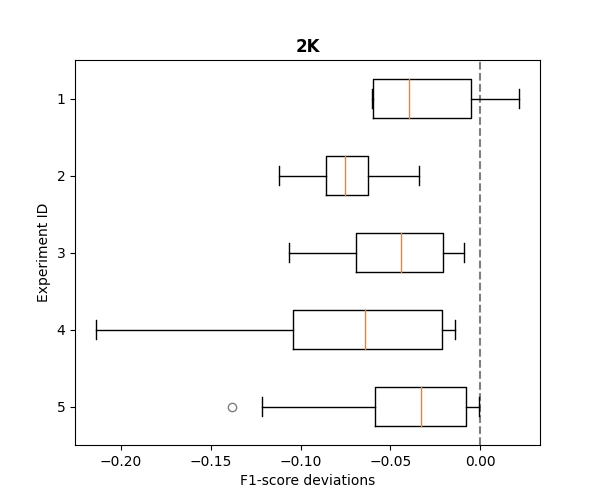
\includegraphics[width=0.5\textwidth]{report/boxplots_2K.png}
    \caption{$F_1$-score deviations from baseline (direct domain transfer A\textrightarrow C) for experiments on 2K.}
    \label{fig:box_2k}
\end{figure}
\begin{figure}[h]
    \centering
    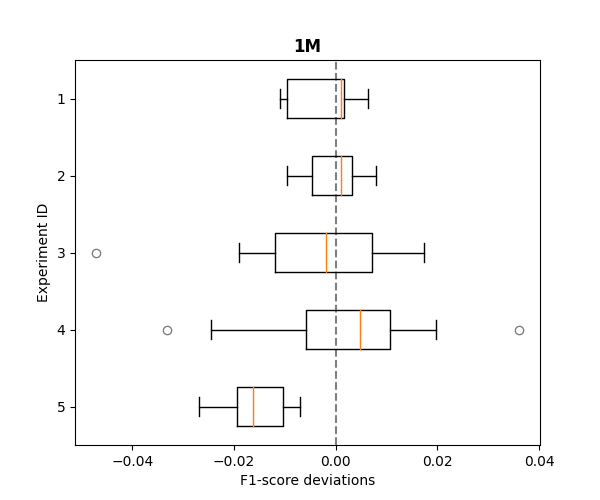
\includegraphics[width=0.5\textwidth]{report/boxplots_1M.png}
    \caption{$F_1$-score deviations from baseline (direct domain transfer A\textrightarrow C) for experiments on 1M.}
    \label{fig:box_1M}
\end{figure}
As can be seen in figure \ref{fig:box_2k} there is a significant performance loss in the 2K experiment, when including intermediate data, as compared to the baseline (dashed).
For figure \ref{fig:box_1M} the price of including this unnecessary intermediate data, does not seem to have a reliably negative effect on performance. Note that the x-axes for the two figures are different scales.

\begin{table}[h]
\centering
\subsection*{\centering 2K Results}
\begin{tabular}{|c|c|c|}
\hline
 \textbf{Experiment} & \textbf{Correlation} & \textbf{\textit{p}-value} \\ \hline
 1 & -0.35 & 0.27 \\ \hline
 2 & -0.18 & 0.57 \\ \hline
 3 & -0.06 & 0.85 \\ \hline
 4 &  0.26 & 0.41 \\ \hline
 5 & -0.05 & 0.88 \\ \hline
\end{tabular}
\caption{Correlation and $p$-values between mean KLD values of the path A \textrightarrow B \textrightarrow C and $F_1$-scores on the target domain.}
\label{tab:corr_2K}
\end{table}
\begin{table}[h]
\centering
\subsection*{\centering 1M Results}
\begin{tabular}{|c|c|c|}
\hline
 \textbf{Experiment} & \textbf{Correlation} & \textbf{\textit{p}-value} \\ \hline
 1 & \,\,0.31 & 0.32 \\ \hline
 2 & -0.18 & 0.58 \\ \hline
 3 & -0.55 & 0.07 \\ \hline
 4 & -0.64 & 0.02 \\ \hline
 5 & -0.16 & 0.62 \\ \hline
\end{tabular}

\caption{Correlation and $p$-values between mean KLD values of the path A \textrightarrow B and B \textrightarrow C and $F_1$-scores on the target domain.}
\label{tab:corr_1M}
\end{table}
Table \ref{tab:corr_2K} and \ref{tab:corr_1M} show Pearson's correlation coefficient and its corresponding $p$-value between mean based KLD and performance. Appendix A contains the results for all three KLD combinations.
We utilize the experiments to test the following hypotheses 
\begin{quote}
    $H_0$ : \textit{"Our combined KLD metric does not correlate with model performance"}
\end{quote}

\begin{quote}
    $H_A$ : \textit{"Our combined KLD metric correlates with model performance"}
\end{quote}

For 2K, the lack of correlation is apparent with $p$-values significantly above 0.05. For 1M the $p$-values also tend to be above 0.05 except for experiment 4.
However, assuming $H_0$ to be true, it is not surprising to see one of our five experiments having a $p$-value of 0.02 or less. The probability of this occurring is about 10\% and thus we do not disregard $H_0$ in favour of $H_A$.
Thus, the tables indicate that there is \textbf{no} a correlation between our domain similarity metric and performance. 

\section*{Discussion}

The experiments seem to show that under certain conditions the intermediate data provides little enough signal to be outweighed by its accompanying noise.
This is not the case for 1M, likely due to the model being able to generalise well from the source domain, thus making it unfazed by the intermediate domain.

However, for 2K we do see a considerable drop in performance as seen in figure \ref{fig:box_2k}. We suspect that for 2K there is not enough data for the model to generalise, so the model mislabels the intermediate domain which only worsens the performance on the target domain.
This indicates that model architectures that are not great for generalisation, or situations where poor or little data is available, can be negatively affected by this method. This aligns well with our intuition.

Furthermore, we do not observe any significant correlation between KLD and performance. This could imply that our method of evaluating domain differences using KLD is flawed.
But, it does seem more likely that the lack of correlation is a consequence of there being no true utility for the bridge, as the domains are too similar. This would leave only noise, which should not be expected to correlate with the KLD.

Assuming the lack of pattern between KLD's and performance, is not due to noise, as we suspect it is, the domain difference evaluation metric would need to be changed. However, this seems unlikely as KLD has shown to be indicative of such differences in the past \cite{van-asch-daelemans-2010-using}.

In conclusion, it seems to be important to quantify the difference between domains, to gauge whether finding additional, intermediate data is useful or not.

\section*{Future work}
One interesting aspect of our results, that we would like explored, is whether the differences in performance of the various intermediate data sets are actually due to noise. Assuming the noise is normally distributed, and that the signal is not, this could be done by measuring the Kolmogorov–Smirnov distance between the errors and the best fitting normal distribution.

In addition to exploring the risks that we have done here, discovering in which particular situations using intermediate data is useful, would be interesting.
As natural languages tend to be quite redundant \cite{yarowsky1995unsupervised}, one would need domains that are significantly more dissimilar than those within the Amazon Review data set, to research this. In this context implementing a method using multiple intermediate data sets, more similar to what is described in \citet{kumar2020understanding}, would be more appropriate.

\section*{Conclusion}
We have seen that using intermediate data to bridge domain differences using self-training, can sometimes have a negative effect if the differences between source and target domains are not sufficiently large.
This is likely because there is enough overlap between the domains, making the intermediate data superfluous, thus only making it a possible source of noise.
This makes it all the more important to quantify the differences between domains accurately. We have attempted the use of Kullback-Leibler divergence as a measure of this, though our experiment was not designed to gauge the usefulness of this particular metric.

\bibliographystyle{acl_natbib}
\bibliography{papers}

%\appendix

\section*{Contributions}
Though initially a part of group 2, Søren Hother Rasmussen (sohr@itu.dk) did not take part in the project. 
As for the rest of us, we did the entire project together either screen-sharing virtually or at ITU campus.
Especially we would like to attribute this project to desktop 10, on the HPC. Fried but not forgotten. . . .



\onecolumn
\newpage
\section*{Appendix A}
\subsection*{\centering 1M Mean \hspace{150} 2K Mean}
\begin{table}[h]
\centering
    \begin{tabular}{|c|c|c|}
    \hline
     \textbf{Experiment} & \textbf{Correlation} & \textbf{\textit{p}-value} \\ \hline
     0 & \,\,0.31 & 0.32 \\ \hline
     1 & -0.18 & 0.58 \\ \hline
     2 & -0.55 & 0.07 \\ \hline
     3 & -0.64 & 0.02 \\ \hline
     4 & -0.16 & 0.62 \\ \hline
    \end{tabular}
\hspace{2em}
    \begin{tabular}{|c|c|c|}
    \hline
     \textbf{Experiment} & \textbf{Correlation} & \textbf{\textit{p}-value} \\ \hline
     1 & -0.40 & 0.19 \\ \hline
     2 & -0.20 & 0.53 \\ \hline
     3 & -0.09 & 0.79 \\ \hline
     4 &  0.16 & 0.61 \\ \hline
     5 & -0.06 & 0.86 \\ \hline
    \end{tabular}
\caption{Correlation and $p$-values between mean bridge KLD values and $F_1$-scores on the target domain, where the bridge score is the mean of the KLD's between A \textrightarrow B and B \textrightarrow C}
\end{table}

\subsection*{\centering 1M Max \hspace{150} 2K Max}
\begin{table}[h]
\centering
    \begin{tabular}{|c|c|c|}
    \hline
     \textbf{Experiment} & \textbf{Correlation} & \textbf{\textit{p}-value} \\ \hline
     0 & 0.38 & 0.22 \\ \hline
     1 & -0.38& 0.23 \\ \hline
     2 & -0.39 & 0.21 \\ \hline
     3 & -0.58 & 0.05 \\ \hline
     4 & -0.16 & 0.61 \\ \hline
    \end{tabular}
\hspace{2em}
    \begin{tabular}{|c|c|c|}
    \hline
     \textbf{Experiment} & \textbf{Correlation} & \textbf{\textit{p}-value} \\ \hline
     0 & -0.59 & 0.04 \\ \hline
     1 & -0.05 & 0.89 \\ \hline
     2 & -0.08 & 0.80 \\ \hline
     3 & -0.18 & 0.58 \\ \hline
     4 & -0.02 & 0.96 \\ \hline
    \end{tabular}
\caption{Correlation and $p$-values between mean bridge KLD values and $F_1$-scores on the target domain, where the bridge score is the max of the KLD's between A \textrightarrow B and B \textrightarrow C}
\end{table}

\subsection*{\centering 1M Harmonic Mean \hspace{100} 2K Harmonic Mean}
\begin{table}[h]
\centering
    \begin{tabular}{|c|c|c|}
    \hline
     \textbf{Experiment} & \textbf{Correlation} & \textbf{\textit{p}-value} \\ \hline
     0 & 0.21 & 0.51 \\ \hline
     1 & -0.12 & 0.72 \\ \hline
     2 & -0.57 & 0.06 \\ \hline
     3 & -0.59 & 0.05 \\ \hline
     4 & -0.16 & 0.62 \\ \hline
    \end{tabular}
\hspace{2em}
    \begin{tabular}{|c|c|c|}
    \hline
     \textbf{Experiment} & \textbf{Correlation} & \textbf{\textit{p}-value} \\ \hline
     0 & -0.33 & 0.30 \\ \hline
     1 & -0.18 & 0.57 \\ \hline
     2 & -0.09 & 0.78 \\ \hline
     3 &  0.26 & 0.42 \\ \hline
     4 & -0.06 & 0.86 \\ \hline
    \end{tabular}
\caption{Correlation and $p$-values between mean bridge KLD values and $F_1$-scores on the target domain, where the bridge score is the harmonic mean of the KLD's between A \textrightarrow B and B \textrightarrow C}
\end{table}

\newpage
\section*{Appendix B}

\begin{table}[h]
\centering
\begin{tabular}{|l|l|l|}
\hline
\textbf{Experiment ID} & \textbf{Source domain} & \textbf{Target domain} \\ \hline
1 & Books & Automotive \\ \hline
2 & Books & Cell Phones and Accessories \\ \hline
3 & Grocery and Gourmet Food & Electronics \\ \hline
4 & Movies and TV & Pet Supplies \\ \hline
5 & Sports and Outdoors & Clothings, Shoes and Jewelry \\ \hline
\end{tabular}
\end{table}



\end{document}